\documentclass[show notes]{beamer}
\usetheme{Rochester}

\usepackage{graphicx}
\usepackage{amsmath,amssymb}
\usepackage{ gensymb }

\title{Advanced Projects in Exoplanets}
\subtitle{The RM Effect}
\author{Dina Sofia Mortensen \& Jesper Dam Knudgaard}
\institute{Stellar Astrophysics Centre, Aarhus University}
\date{\today}

\begin{document}

\begin{frame}
\titlepage
\end{frame}

\section{The RM Effect}

\begin{frame}
\frametitle{Transiting Exoplanets}
	\begin{figure}
		\centering
		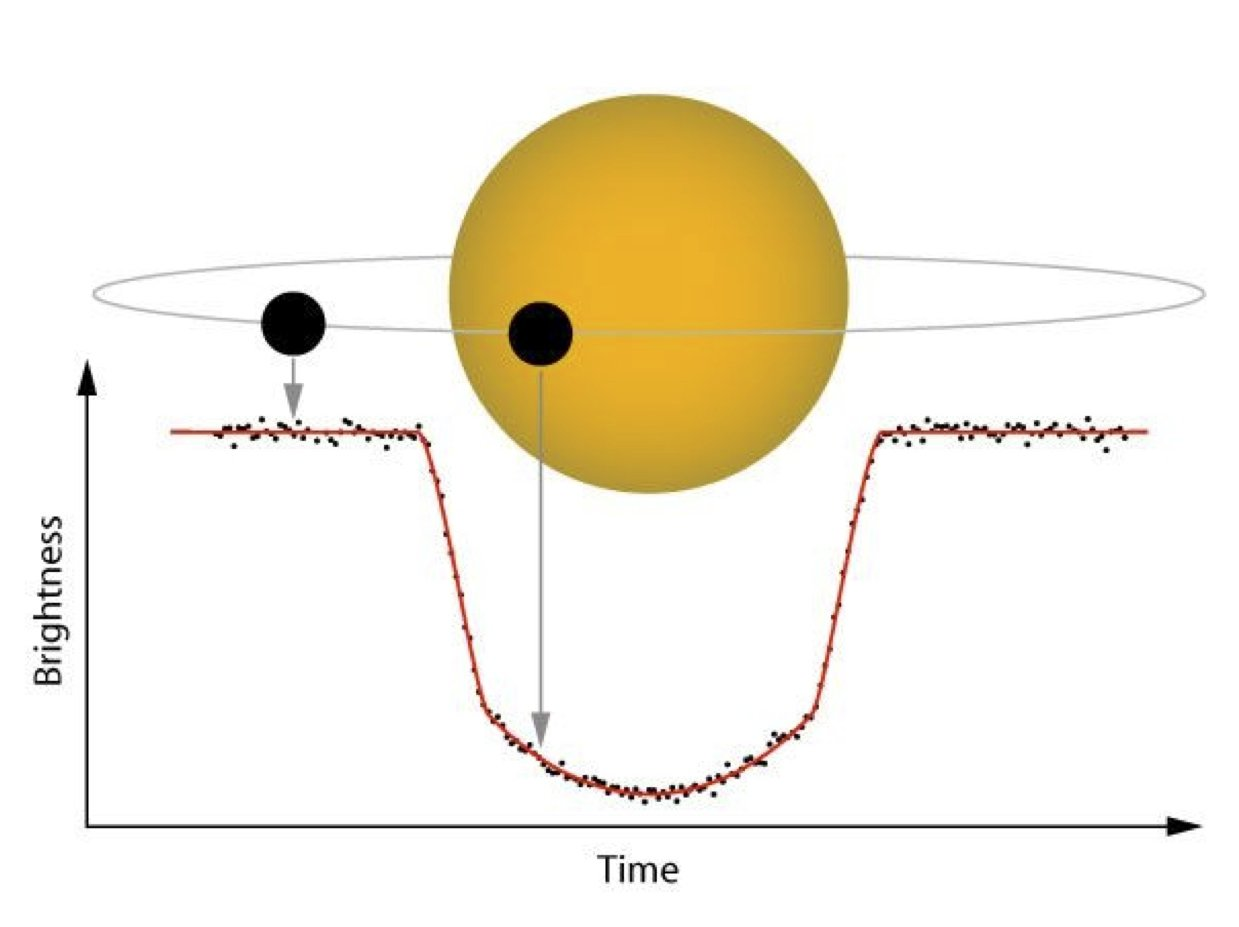
\includegraphics[width = 0.7\columnwidth]{../figures/Transit.jpg}
		\caption{\textit{Credit ESO}}
		\label{fig:transit} 
	\end{figure}
\end{frame}

\begin{frame}
\frametitle{Rossiter-McLaughlin Effect}
	\begin{figure}
		\centering
		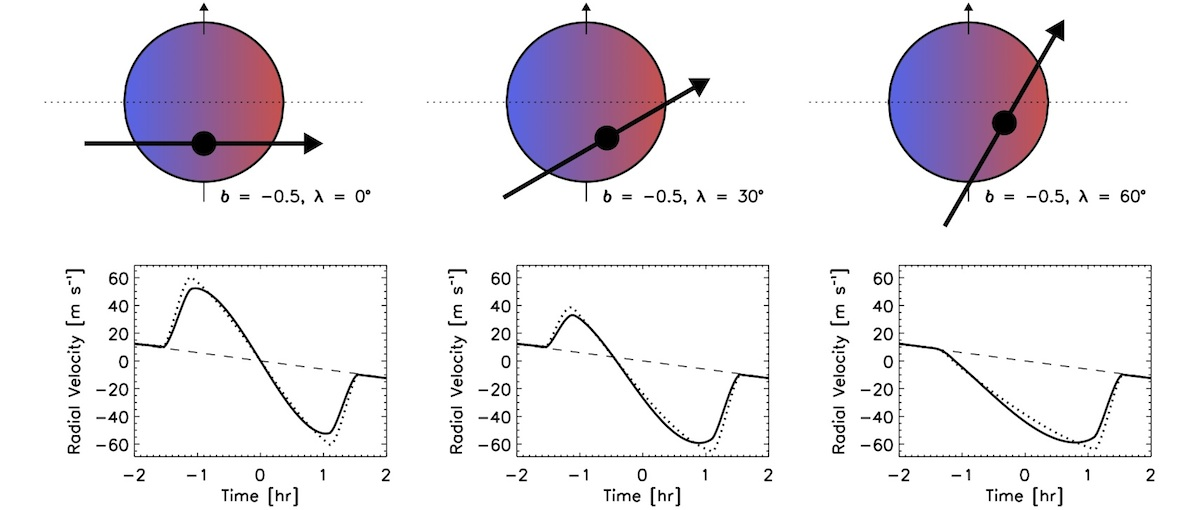
\includegraphics[width=\textwidth]{../figures/winnwhites.jpg}
		\caption{\url{https://wasp-planets.net/tag/rossiter-mclaughlin-effect/}}
		\label{fig:rm_effect}
	\end{figure}
\end{frame}

\note{Husk at nævne at det kun er projiceret obliquity vi kan måle, og det er fordi vi ikke ved hvordan stjernens rotationsakse er inklineret i forhold til os. }

\begin{frame}
\frametitle{}

\end{frame}

\section{Our Model}

\begin{frame}
\frametitle{Our Model - Linear}
\begin{columns}
	\column{0.5\textwidth}
		Planet moves in straight line in front of the star\\
		
		This path is determined by:
		\begin{itemize}
			\item Projected obliquity
			\item Impact parameter
		\end{itemize}
		
		This model is not physical
		
	\column{0.5\textwidth}

\end{columns}
\end{frame}


\begin{frame}
\frametitle{Keplers Equations}	
	
\end{frame}


\begin{frame}
\frametitle{Our Model - Physical version}
\begin{columns}
	\column{0.5\textwidth}
		Planet orbits the star.\\
		
		Keplers equation is solved for input parameters.\\

		The path is determined by:\\
		 $ a $, $ e $, $ i $, $ \omega $, $ M_{\star} $, $ M_p $, $ t_p $, $ \lambda $, $ R_p/R_{\star} $ and $ v\sin(i) $.\\
		
		Much more resource heavy, but also correct
		
	\column{0.5\textwidth}
		\begin{figure}
			\centering
			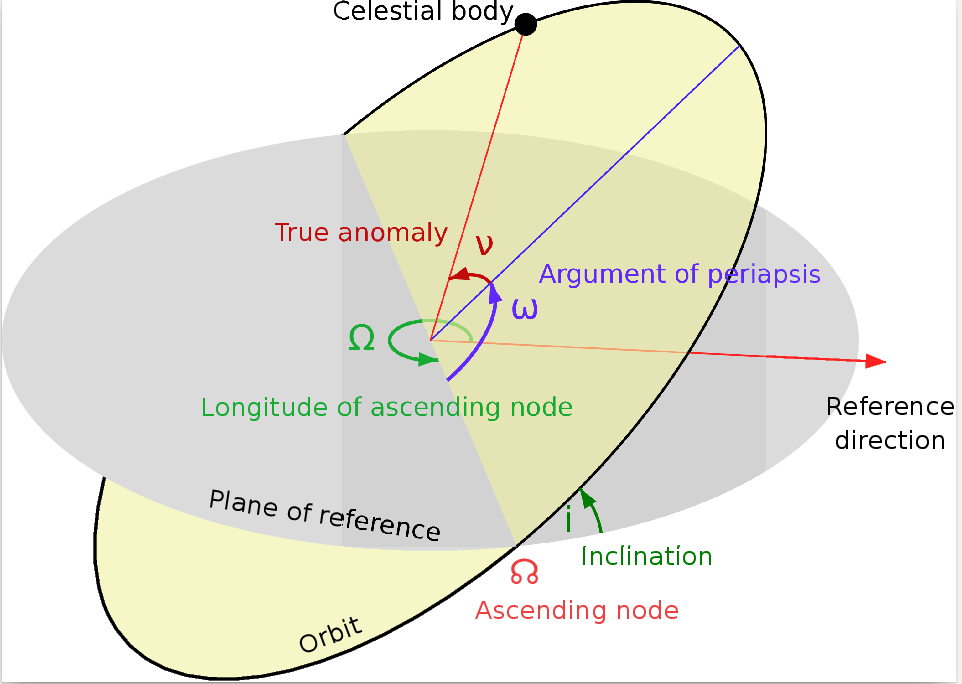
\includegraphics[width=\textwidth]{../figures/kepler.png}
			\caption{Credit: Wikipedia user Lassuncty}
			\label{fig:orbit}
		\end{figure}
\end{columns}

\end{frame}

\note{Vi laver her antagelsen at transit midpunkt sker til tiden t=0, og at $ \omega=90 $, så i tilfældet hvor vi har en eccentricitet, vil transitten ske ved periapsis.}

\begin{frame}
\frametitle{Our Model - Outputs}
	[Video here]
\end{frame}

\begin{frame}
\frametitle{Our Model - Outputs}

Så her tænker jeg at vi har selve RM-kurven. Så vi snakker noget om hvor fucked Gauss fittet er
\end{frame}

\begin{frame}
\frametitle{Data}
\begin{columns}
	\column{0.5\textwidth}
	
	
	\column{0.5\textwidth}
	\begin{figure}
		\centering
		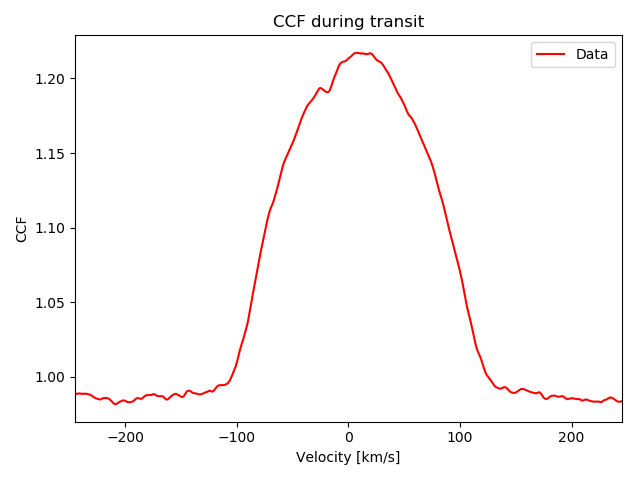
\includegraphics[width=\textwidth]{../figures/CCF_it.png}
		\label{fig:CCF_it}
	\end{figure}	
\end{columns}
\end{frame}

\begin{frame}
\frametitle{Data - The stellar line}
\begin{figure}
	\centering
	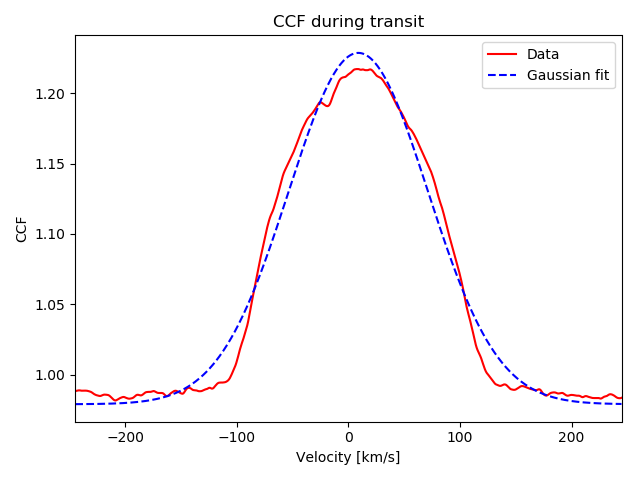
\includegraphics[width=0.8\textwidth]{../figures/CCF_it_fit.png}
	\label{fig:CCF_fit}
\end{figure}
\end{frame}

\begin{frame}
\frametitle{Data - The Transit}
\begin{figure}
	\centering
	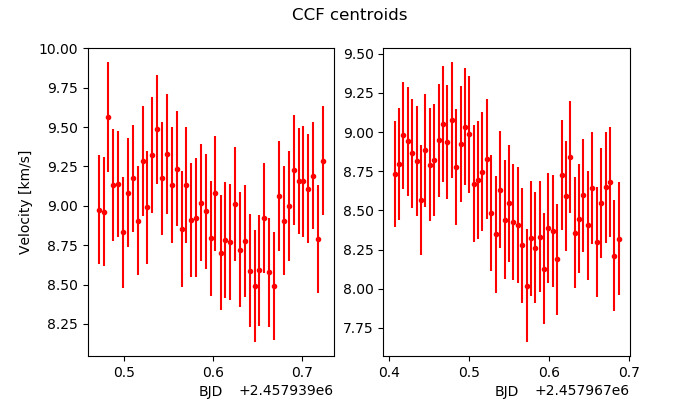
\includegraphics[width=\textwidth]{../figures/ccf_centroids.png}
	\label{fig:CCF_cent}
\end{figure}
\end{frame}

\begin{frame}
\frametitle{Data - The 'Planet Line'}
\begin{figure}
	\centering
	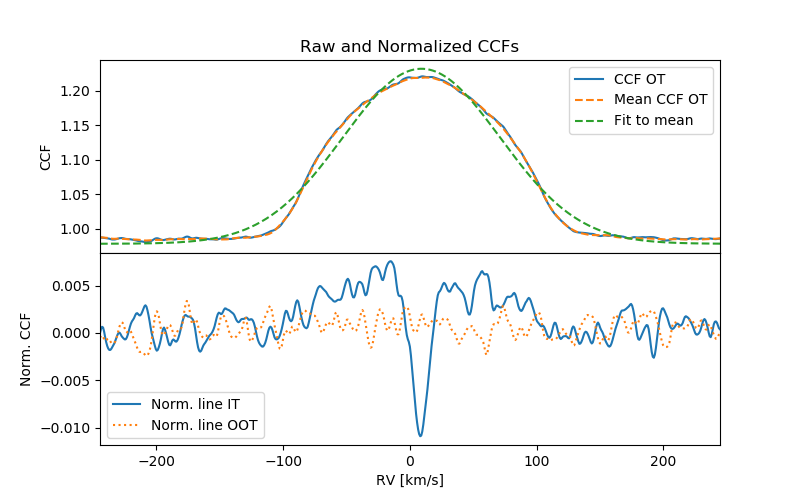
\includegraphics[width=\textwidth]{../figures/ccfs_norm.png}
	\label{fig:CCFs_norm}
\end{figure}
\end{frame}

\begin{frame}
\frametitle{Data - The RM-effect}
	\begin{figure}
	\centering
%	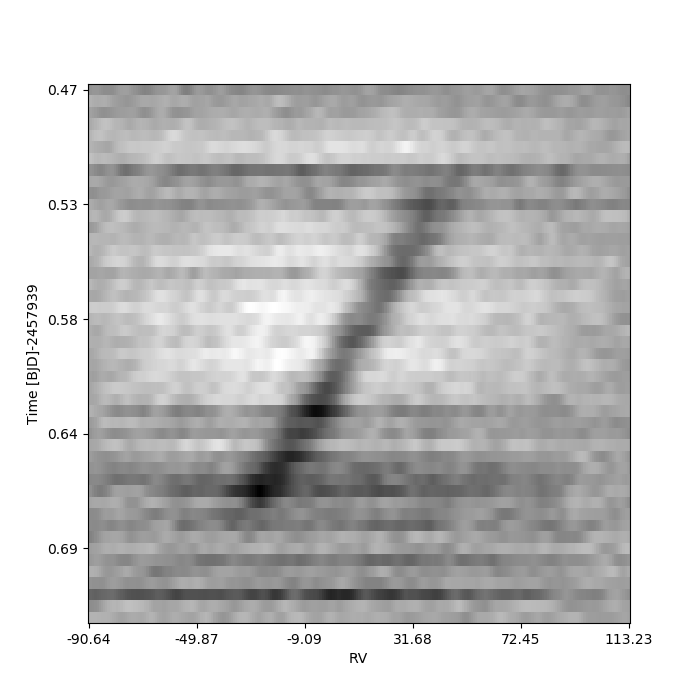
\includegraphics[width=\textwidth]{../figures/Colormap.png}
	\label{fig:colormap}
\end{figure}
\end{frame}


\begin{frame}
\frametitle{Data}
	\begin{figure}
	\centering
	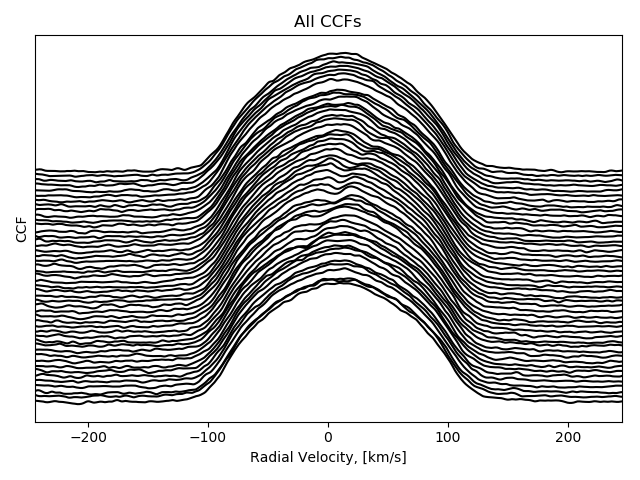
\includegraphics[width=0.8\textwidth]{../figures/All_CCFs.png}
	\label{fig:all_ccfs}
\end{figure}
\end{frame}


\begin{frame}
\frametitle{Data - Fit to CCF}
\begin{figure}
	\centering
	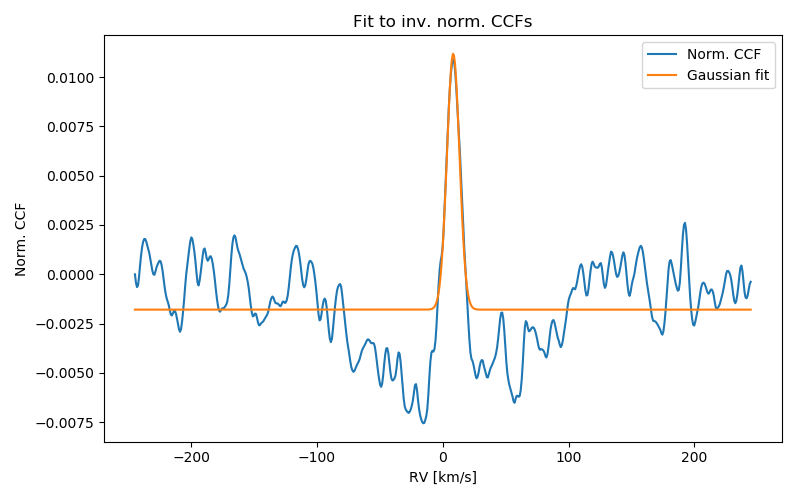
\includegraphics[width=\textwidth]{../figures/fitted_ccf.png}
	\label{fig:fitted_ccf}
\end{figure}
\end{frame}

\begin{frame}
\frametitle{Data - RM curve}
	\begin{figure}
		\centering
		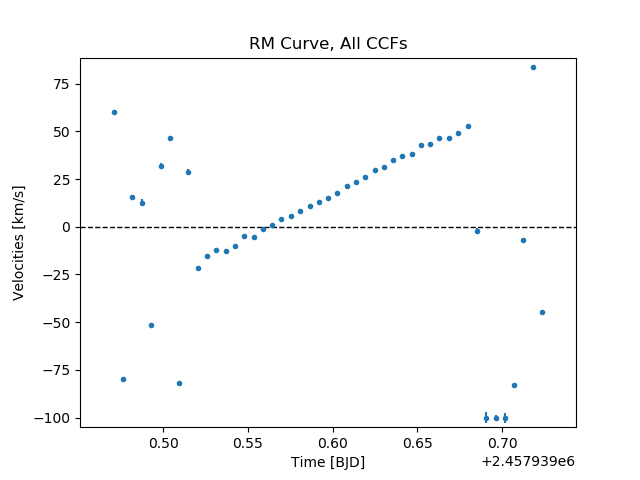
\includegraphics[width=0.8\textwidth]{../figures/RM_all_CCFs.png}
		\label{fig:RM_all_CCFs}
	\end{figure}
\end{frame}


\begin{frame}
\frametitle{Data - RM curve}
\begin{figure}
	\centering
	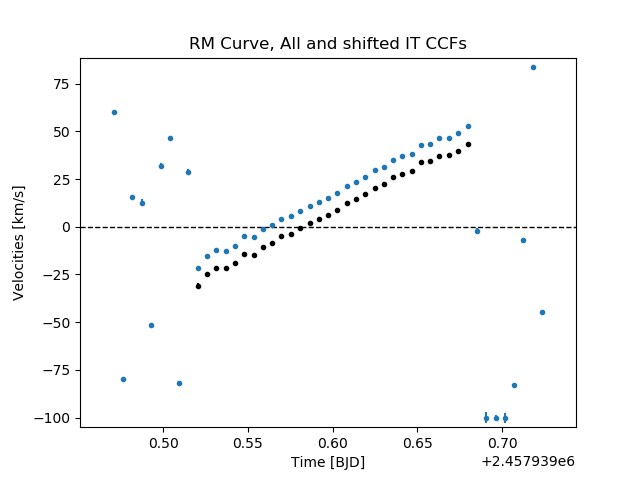
\includegraphics[width=0.8\textwidth]{../figures/RM_all_shift.png}
	\label{fig:RM_all_shift}
\end{figure}
\end{frame}

\begin{frame}
\frametitle{Data - RM curve}
\begin{figure}
	\centering
	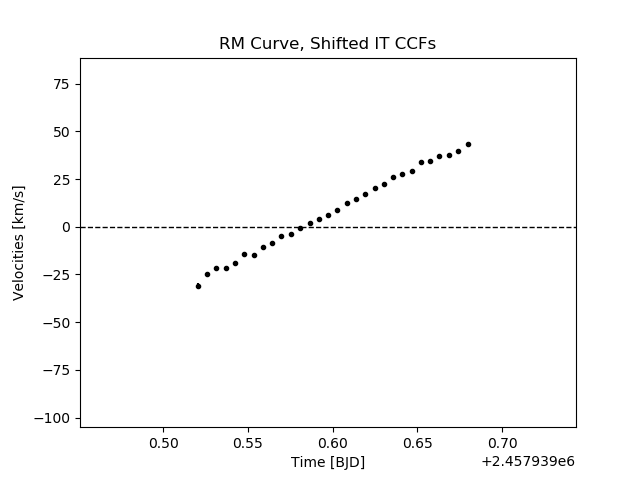
\includegraphics[width=0.8\textwidth]{../figures/RM_shift.png}
	\label{fig:RM_shift}
\end{figure}
\end{frame}

\section*{The Fit}

\begin{frame}
\frametitle{The Fit - System Parameters}

\end{frame}

\begin{frame}
\frametitle{Fitting with curvefit}

\end{frame}

\begin{frame}
\frametitle{Linear fit}
\end{frame}


\end{document}
